\parindent=0em
\subsection{Atención médica}
\noindent

%https://blogs.windows.com/windowsexperience/2018/03/08/how-mixed-reality-is-changing-the-game-for-healthcare-from-performing-live-surgeries-to-delivering-ultrasounds-in-3d/

Existen diversos usos de la realidad mixta en la atención médica, en primer lugar, la empresa \textit{CAE Healthcare} es una de las líderes en simulaciones tecnológicas y en recursos para mejorar el desempeño en las clínicas. \textit{CAE VimedixAR} es un simulador de ultrasonido diseñado por dicha empresa para las \textit{HoloLens}, de esta forma, los profesionales pueden manipular partes anatómicas (rotándolas y escalándolas).\\

Otra aplicación diseñada por esta empresa es \textit{CAE Lucina} (figura \ref{fig:caelucina}). Se trata de un simulador de partos donde los profesionales pueden realizar la extracción completa del feto en cualquier situación excepcional (estando así preparados para cualquier imprevisto).

\begin{figure}[h]
    \centering
    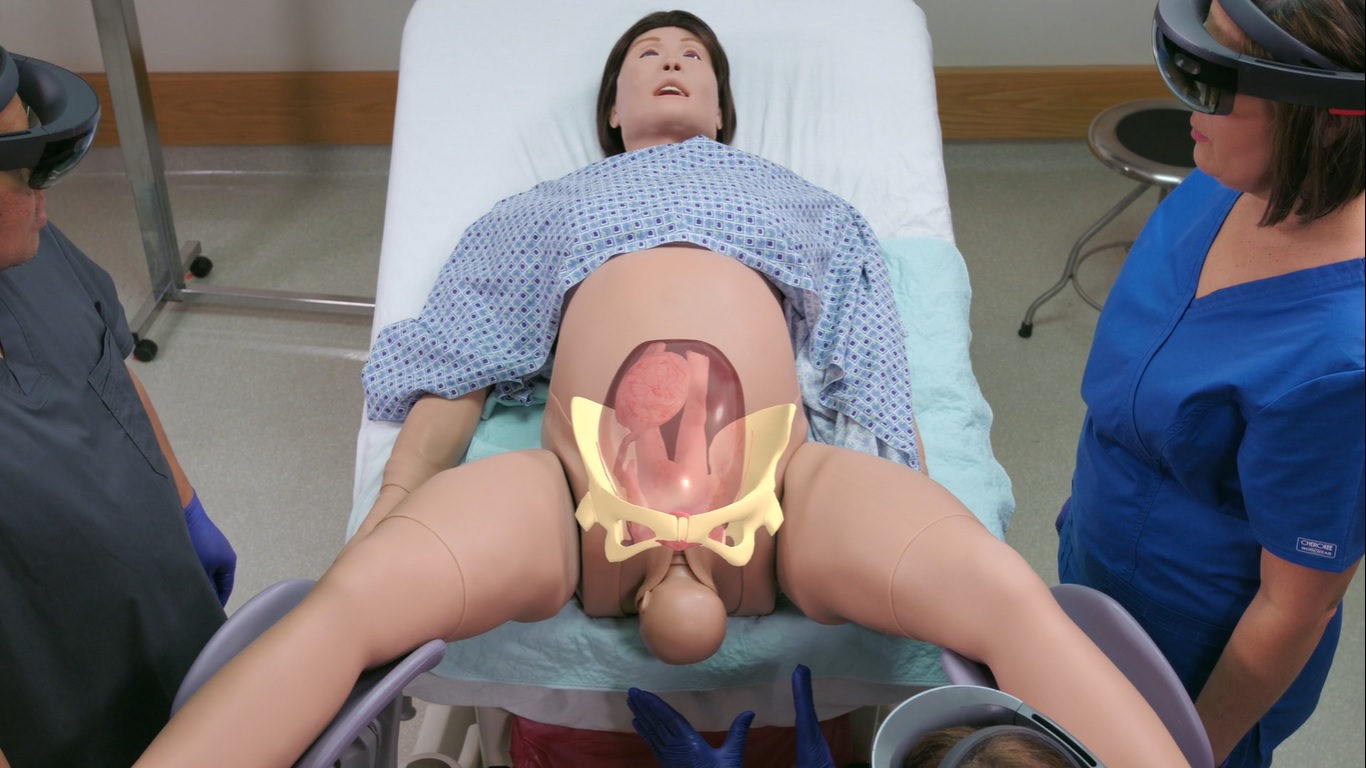
\includegraphics[scale=0.38]{Images/Estado del arte/caehealthcareparto.jpg}
    \caption{CAE Lucina en ejecución con las HoloLens.}
    \label{fig:caelucina}
\end{figure}

Por otro lado, la empresa \textit{Pearson} ha desarrollado una aplicación llamada \textit{HoloPatient} la cual sirve para formar estudiantes de enfermería. El programa se basa en una experiencia que permite aprender sin necesidad de actores o pacientes que se necesitarían sin usar esta tecnología. \textit{HoloPatient} salió al mercado en Abril del año 2018.\\

Existen otros proyectos como el que viene de la mano de \textit{SphereGen} en colaboración con una universidad, bautizado con el nombre de \textit{Learning Heart} (figura \ref{fig:learningheartspheregen}). Esta aplicación enfocada a su uso a través de las \textit{HoloLens}, permite a sus usuarios aprender sobre el corazón (de manera individual o colaborativa) viéndolo desde cualquier ángulo y posición. 

\begin{figure}[h]
    \centering
    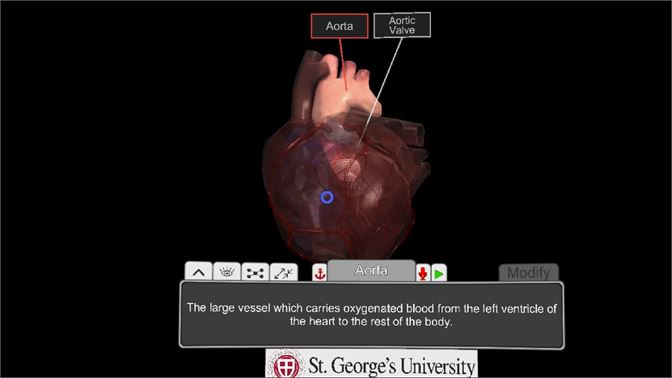
\includegraphics[scale=0.65]{Images/Estado del arte/learningheartspheregen.jpeg}
    \caption{\textit{Learning Heart} en ejecución.}
    \label{fig:learningheartspheregen}
\end{figure}


%Foto del learning 
%https://www.microsoft.com/en-us/p/learning-heart/9pghzvfwxpmb?activetab=pivot:overviewtab}


En cuanto a la radiología, \textit{DICOM Director} aporta una gran ayuda a estos expertos permitiéndoles ver y analizar todo tipo de escaneos en 3D. Los radiólogos y doctores pueden ver estas radiografías haciendo uso de sus \textit{HoloLens} o sus cascos de realidad mixta de Windows, igualmente, la aplicación genera un modelo 3D de esas imágenes (figura \ref{fig:dicomDirector}) los cuales se pueden rotar y analizar. De esta manera, \textit{DICOM Director} se utiliza también como herramienta de comunicación entre doctores para compartir estos modelos.

\begin{figure}[h]
    \centering
    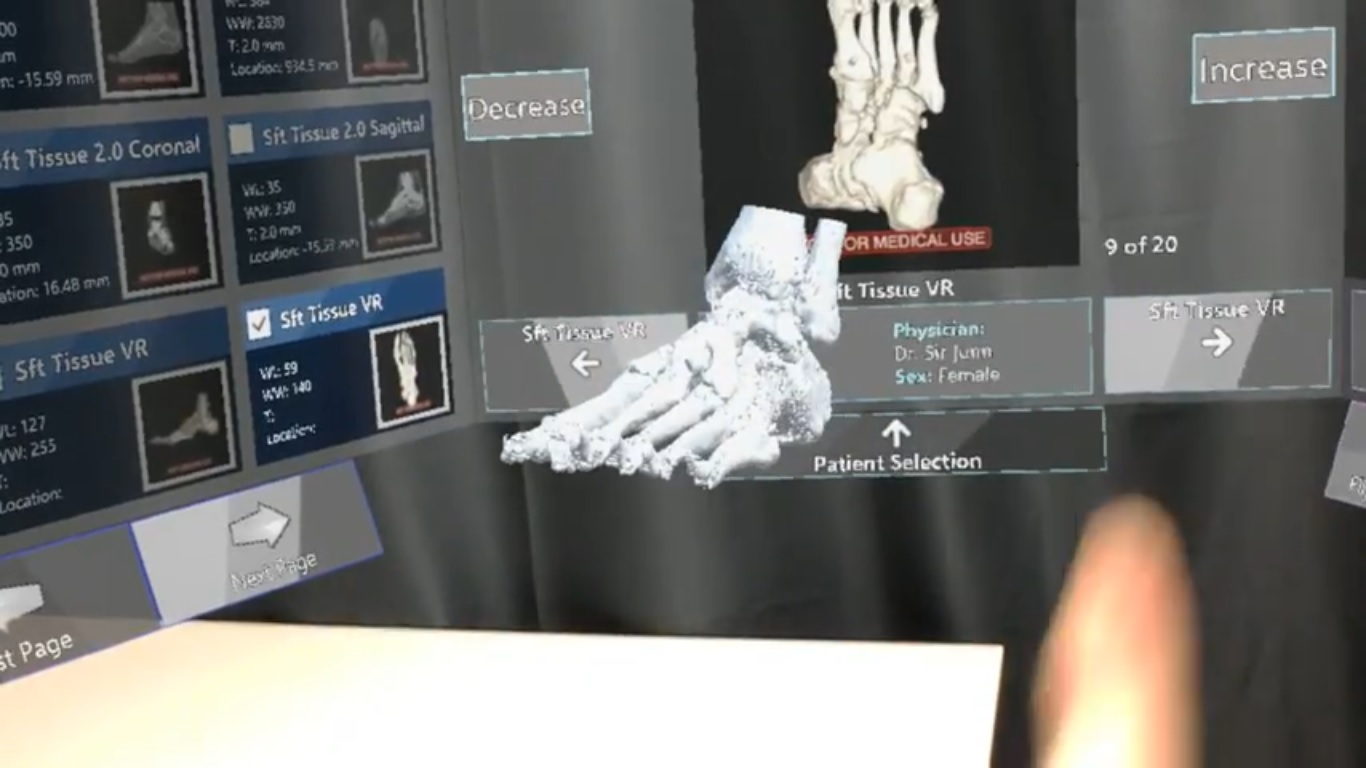
\includegraphics[scale=0.25]{Images/Estado del arte/dicomdirector.jpg}
    \caption{Usuario rotando el modelo 3D de una radiografía en\textit{DICOM Director}.}
    \label{fig:dicomDirector}
\end{figure}

Para finalizar, la empresa \textit{Visual 3D Medical Science and Technology Development CO. LLC} ha desarrollado un producto que ha sido usado en China para realizar 200 operaciones (de rodilla, cadera y espina) gracias a la realidad mixta. Incluso se está utilizando para preparar a los cirujanos antes de entrar a la sala de operaciones, reproduciendo la operación a través de las gafas. 






